\documentclass[aspectratio=169, table]{beamer}

%\usepackage[beamertheme=./praditatheme]{Pradita}

\usetheme{Pradita}

\subtitle{MTI102-Information System \&\\Technology Architecture}
\title{\vskip-0.7cm \Large Phase E: Opportunities and Solutions\\in TOGAF
	Architecture\\Development Method (ADM)}
\date[Serial]{\scriptsize {PRU/SPMI/FR-BM-18/0222}}
\author[Pradita]{\small {\textbf{Alfa Yohannis}}}

\begin{document}
	
	\frame{\titlepage}
	
	\begin{frame}
		\frametitle{Aims}
		\begin{enumerate}
			\item Generate the initial complete version of the Architecture Roadmap, based upon the gap analysis and candidate Architecture Roadmap components from Phases B, C, and D.
			\item Determine whether an incremental approach is required, and if so identify Transition Architectures that will deliver continuous business value.
		\end{enumerate}
		
	\end{frame}
	
	\begin{frame}
		\frametitle{Inputs (1)}
		\vspace{20pt}
		\begin{columns}[onlytextwidth]
			\begin{column}{0.45\textwidth}
				\begin{enumerate}
					\item Product information
					\item Request for Architecture Work
					\item Capability Assessment
					\item Communications Plan
					\item Planning Methodologies
					\item Organizational Model for Enterprise Architecture
					\item Governance Models and Frameworks
					\item Tailored Architecture Framework
				\end{enumerate}
				
			\end{column}
			\begin{column}{0.55\textwidth}
				\begin{enumerate}
					\setcounter{enumi}{8}
					\item Statement of Architecture Work
					\item Architecture Vision
					\item Architecture Repository
					\item Draft Architecture Definition Document
					\item Draft Architecture Requirements Specification
					\item Change Requests for existing programs and projects
					\item Candidate Architecture Roadmap components from Phases B, C, and D
				\end{enumerate}
			\end{column}
		\end{columns}
	\end{frame}
	
	
	\begin{frame}
		\frametitle{Steps}
		\vspace{20pt}
		\begin{columns}[onlytextwidth]
			\begin{column}{0.50\textwidth}
				\begin{enumerate}
					\item Determine/confirm key corporate change attributes
					\item Determine business constraints for implementation
					\item Review and consolidate Gap Analysis results from Phases B to D
					\item Review consolidated requirements across related business functions
					\item Consolidate and reconcile interoperability requirements
					
				\end{enumerate}
				
			\end{column}
			\begin{column}{0.50\textwidth}
				\begin{enumerate}
					\setcounter{enumi}{5}
					\item Refine and validate dependencies
					\item Confirm readiness and risk for business transformation
					\item Formulate Implementation and Migration Strategy
					\item Identify and group major work packages
					\item Identify Transition Architectures
					\item Create the Architecture Roadmap \& Implementation and Migration Plan
				\end{enumerate}
			\end{column}
		\end{columns}
	\end{frame}
	
	\begin{frame}
		\frametitle{Steps (1)}
		\vspace{20pt}
		\begin{itemize}
			\item \textbf{Determine/confirm key corporate change attributes}
			\begin{itemize}
				\item Asses the transition capabilities of enterprise (including culture and abilities) documented into the Implementation Factor Assessment and Deduction matrix
				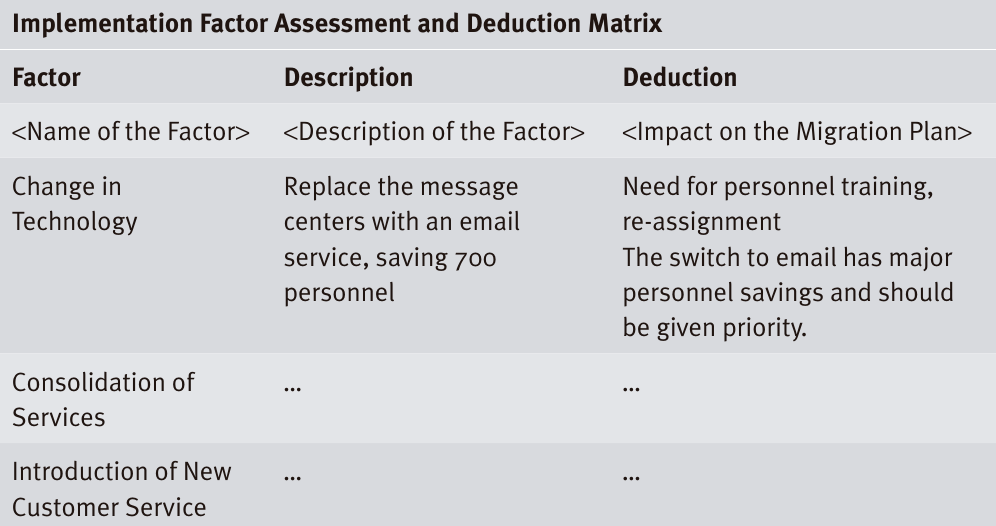
\includegraphics[width=0.6\textwidth]{../figures/factor_assessment_and_deduction_matrix.png}			
			\end{itemize}
		\end{itemize}
	\end{frame}

	\begin{frame}
		\frametitle{Steps (2)}
		\vspace{20pt}
		\begin{itemize}
			\item \textbf{Determine Business Constraints for Implementation}
			\begin{itemize}
				\item Identify any business drivers that would constrain the sequence of
				implementation.
			\end{itemize}
		\end{itemize}
	\end{frame}

	\begin{frame}
		\frametitle{Steps (3)}
		\vspace{20pt}
		\begin{itemize}
			\item \textbf{Review and consolidate Gap Analysis results from Phases B to D}
			\begin{itemize}
				\item Consolidate and integrate the Gap Analysis results from the Business, Information Systems, and Technology Architectures 
				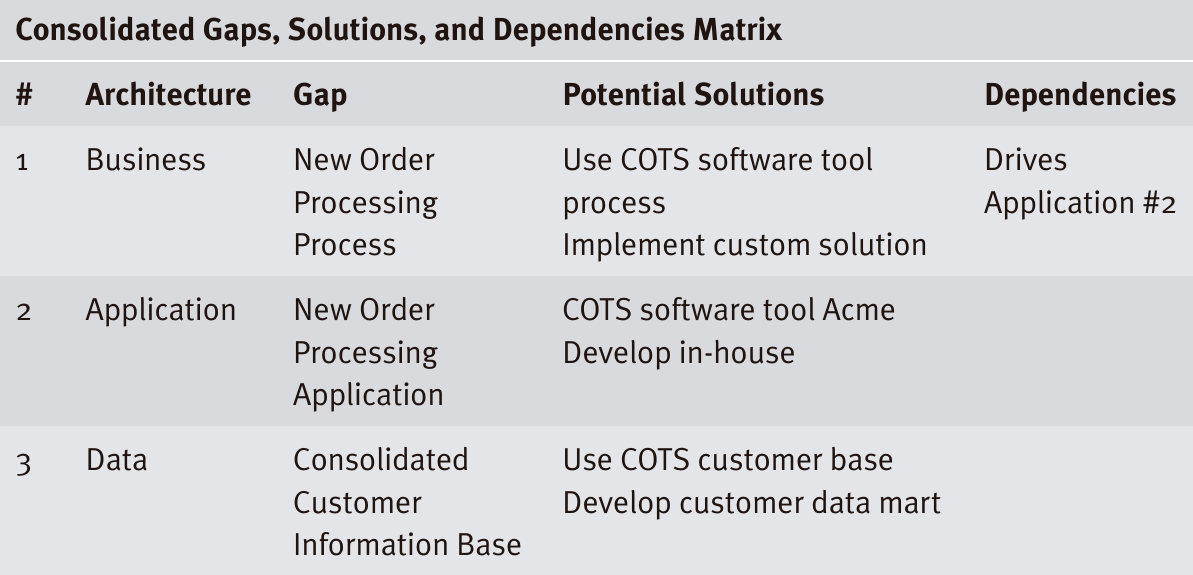
\includegraphics[width=0.6\textwidth]{../figures/consolidated_gaps_solutions_and_depedencies_matrix.png}			
			\end{itemize}
		\end{itemize}
	\end{frame}

	\begin{frame}
		\frametitle{Steps (4)}
		\vspace{20pt}
		\begin{itemize}
			\item \textbf{Review Consolidated Requirements Across Related Business Functions}
			\begin{itemize}
				\item Assess the requirements, gaps, solutions, and factors across the business functions.
				\item Integrate them into work packages to create an
				efficient and effective implementation of the Target Architecture. 
				\item Satisfy multiple requirements through the provision of shared solutions and services. 
				\item Optimise the provision of resources. 
				\item For example, several
				requirements raised by several lines of business can be resolved through
				the provision of a shared set of Business Services and Information System
				Services within a work package or project.
				
			\end{itemize}
		\end{itemize}
	\end{frame}

	\begin{frame}
		\frametitle{Steps (5)}
		\vspace{20pt}
		\begin{itemize}
			\item \textbf{Consolidate and Reconcile Interoperability Requirements}
			\begin{itemize}
				\item Implementation Factor Assessment and Deduction matrix and Consolidated
				Gaps, Solutions, and Dependencies matrix, should be consolidated and
				reviewed.
				\item To identify any constraints on interoperability required by the
				potential set of solutions. 
				\item A key outcome is to minimize interoperability conflicts
				\item Re-used Solution Building Blocks, Commercial Off-The-Shelf
				(COTS) products, and third-party service providers typically impose
				interoperability requirements that conflict.
			\end{itemize}
		\end{itemize}
	\end{frame}

	\begin{frame}
		\frametitle{Steps (6)}
		\vspace{20pt}
		\begin{itemize}
			\item \textbf{Refine and Validate Dependencies}
			\begin{itemize}
				\item Dependencies should be used for determining
				the sequence of implementation and identifying the coordination required.
				\item  Dependencies should group activities together, creating a basis
				for projects to be established.
				\item  The dependencies also help to identify when the identified increment can be delivered.
			\end{itemize}
		\end{itemize}
	\end{frame}

	\begin{frame}
		\frametitle{Steps (7)}
		\vspace{20pt}
		\begin{itemize}
			\item \textbf{Confirm Readiness and Risk for Business Transformation}
			\begin{itemize}
				\item The architects should review the Readiness Assessment conducted in Phase A and determine their
				impact on the Architecture Roadmap and the Implementation and Migration
				Strategy. 
				\item It is important to identify, classify, and mitigate risks associated with
				the transformation effort. 
				\item Risks should be documented in the Consolidated
				Gaps, Solutions, and Dependencies matrix.
			\end{itemize}
		\end{itemize}
	\end{frame}

	\begin{frame}
		\frametitle{Steps (8)}
		\vspace{20pt}
		\begin{itemize}
			\item \textbf{Formulate Implementation and Migration Strategy}
			\begin{itemize}
				\item \textbf{Greenfield}. A completely new implementation.
				\item \textbf{Revolutionary}. A radical change (i.e., switch on, switch off ).
				\item \textbf{Evolutionary}. A strategy of convergence, such as parallel running or a
				phased approach to introduce new capabilities.
				\item Also determine solutions to mitigate identified risks
			\end{itemize}
		\end{itemize}
	\end{frame}

		\begin{frame}
		\frametitle{Steps (9)}
		\vspace{20pt}
		\begin{itemize}
			\item \textbf{Identify and Group Major Work Packages}
			\begin{itemize}
				\item Group the various activities into work packages 
				\item work package is an inter-dependent set of activities and deliverables that deliver a discrete
				enterprise outcome
				\item Solution should be oriented towards a new development, based upon an existing product, and/or
				use a solution that can be purchased
				\item Classify every current system as Mainstream (part of the future information system), Contain (expected to be replaced or modified in the planning horizon, e.g., next three years), Replace (to be replaced in the planning horizon).
			\end{itemize}
		\end{itemize}
	\end{frame}

	\begin{frame}
		\frametitle{Steps (10)}
		\vspace{20pt}
		\begin{itemize}
			\item \textbf{Identify Transition Architectures}
			\begin{itemize}
				\item Where the scope of change to implement the Target Architecture requires an incremental approach, then one or more Transition
				Architectures may be necessary. 
				\item These provide an ability to identify clear
				targets along the roadmap to realizing the Target Architecture. 
				\item The Transition Architectures should provide measurable business value
			\end{itemize}
		\end{itemize}
	\end{frame}

		\begin{frame}
		\frametitle{Steps (11)}
		\vspace{20pt}
		\begin{itemize}
			\item \textbf{Create the Architecture Roadmap \& Implementation and Migration Plan (Outline)}
			\begin{itemize}
				\item Consolidate the work packages and Transition Architectures into the
				Architecture Roadmap
				\item It describes a timeline of the
				progression from the Baseline Architecture to the Target Architecture
			\end{itemize}
		\end{itemize}
	\end{frame}
	
	\begin{frame}
		\frametitle{Outputs}
		\vspace{25pt}
		\begin{columns}[onlytextwidth]
			\begin{column}{0.50\textwidth}
				\begin{enumerate}
					\item Statement of Architecture Work, updated if necessary
					\item Architecture Vision, updated if necessary
					\item Draft Architecture Definition Document, updated if necessary, including:
					\begin{itemize}
						\item Transition Architectures, if any
					\end{itemize}
					\item Draft Architecture Requirements Specification, including:
					\begin{itemize}
						\item Consolidated Gaps, Solutions, and Dependencies Assessment
					\end{itemize}
				\end{enumerate}
				
			\end{column}
			\begin{column}{0.50\textwidth}
				\begin{enumerate}
					\setcounter{enumi}{4}
					\item Capability Assessment, including:
					\begin{itemize}
						\item Business Capability Assessment
						\item IT Capability Assessment
					\end{itemize}
					\item Architecture Roadmap, including:
					\begin{itemize}
						\item Work package portfolio
						\item Identification of Transition Architectures, if any
						\item Implementation recommendations
					\end{itemize}
					\item Implementation and Migration Plan (outline)
				\end{enumerate}
			\end{column}
		\end{columns}
	\end{frame}
	
	
	\begin{frame}
		\frametitle{Summary}
		\begin{enumerate}
			\item The Opportunity and Solutions Phase allows us to identify and develop effective and efficient architectural solutions. 
			\item It helps in planning the detailed implementation of the architecture.
		\end{enumerate}
	\end{frame}
	
\end{document}`